% Условная компиляция для самостоятельной работы
\ifdefined\mainfile
    % Если это часть основного файла, не добавляем начало и конец документа
\else
    \documentclass[12pt, a4paper]{report}
    \usepackage{/Users/vladbelousov/Desktop/Semestr_4-FP-NSU/Настройка/library}
    \usepackage[utf8]{inputenc} % Подключение поддержки UTF-8
    \begin{document}
\fi

%%-------------------------------%%

\textbf{Второе уравнение Максвелла:}

\[ \mathrm{rot } (\vec{H_0 }(\vec{r } ) e^{ i k_0 \psi (\vec{r } )- i \omega t }) = -\frac{i \omega  \varepsilon}{c } \vec{E } _0 e^{ i k_0 \psi - i \omega t }         \] 

\[ \mathrm{rot } \vec{H } _0 e^{i k_0 \psi(\vec{r} ) - i \omega t    }  + i k_0 [\nabla \psi (\vec{r } \times  \vec{H}  _0 )]e^{i k_0 \psi(\vec{r } )- i \omega t} = - \frac{i \omega \varepsilon(\vec{r } )}{c } \vec{E } _0 (\vec{r } ) e^{ i k_0 \psi(\vec{r } )- i \omega t }    \] 

\[ \Rightarrow [\nabla \psi (\vec{r } )\times  \vec{H } _0 (\vec{r } )] = - \varepsilon (\vec{r } ) \vec{E } _0 (\vec{r } ) \Rightarrow [\nabla \psi (\vec{r } ) \times  \vec{B } _0 (\vec{r } )] = - \varepsilon(\vec{r } ) \mu(\vec{r} ) \vec{E } _0 (\vec{r} )\] 

\textbf{Продолжение вектора Умова-Пойтинга}: 

\[ <\vec{\mathbb{S}}> = \frac{c}{8 \pi } [ \vec{E } \times  \vec{H }^*   ]   = \frac{c}{8 \pi } \mathrm{Re } [ \vec{E } _0 (\vec{r } )e^{ i k_0 \psi( \vec{r } )- i \omega t }\times  \vec{H } _0 ^* e^{ -i k_0 \psi(\vec{r } ) + i\omega t }  ]  \] 

\[ \text{Подставим: } \nabla \psi(\vec{r }  \times  \vec{E } _0 (\vec{r } )) = \vec{B } _0 (\vec{r } ) \] 

\[ <\vec{\mathbb{S} } > = \frac{c}{\mu(\vec{r } ) 8 \pi } [\vec{E } _0 (\vec{r }  )\times  [ \nabla \psi(\vec{r } ) \times  \vec{E } _0 ^ * (\vec{r } )]] = \frac{c}{\mu(\vec{r } )8 \pi } \mathrm{Re } \{ \nabla \psi (\vec{E } _0 (\vec{r }) , \vec{E} _0 ^* ) - ( \nabla\psi , \vec{E } _0 ^ * (\vec{r } )) \vec{E } _0 ^* (\vec{r } ) \} =  \] 

\[ = \underbrace{\frac{c}{\sqrt{\varepsilon (\vec{r }  )\mu (\vec{r } )}}}_{v_{\Phi} } \underbrace{\frac{\nabla \psi }{\sqrt{\varepsilon (\vec{r } )\mu (\vec{ r } )} } }_{|\nabla  \psi | = \sqrt{\varepsilon \mu } = n \text{ } (1)}\underbrace{\frac{ \varepsilon \left\lvert \vec{E } _0    \right\rvert ^2 }{ 8 \pi }}_{2W_E = W_E + W_B}  = \frac{c}{\sqrt{\varepsilon \mu }}\vec{u } (W_E + W_B)   \] 

(1) - единичный вектор вдоль \( \nabla \psi   \), вдоль луча \( \vec{u}  \)

\textbf{Уравнение для луча: } 

\begin{center}
    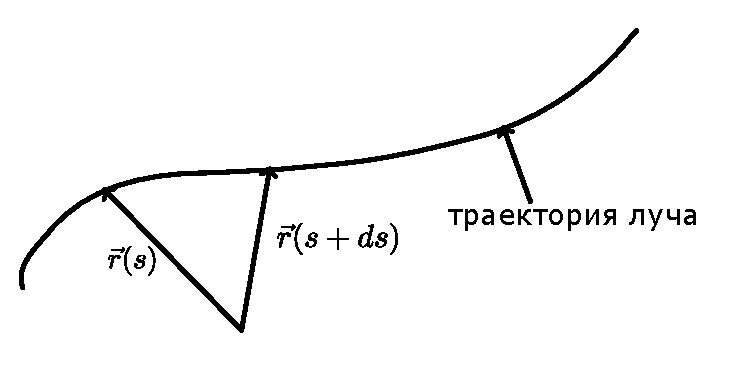
\includegraphics[width=0.5\textwidth]{/Users/vladbelousov/Desktop/Semestr_4-FP-NSU/ЭиО/Лекции_по_дням/image/65.pdf}
\end{center}

\[ \frac{d \vec{r } }{ds}   = \frac{\vec{r } (s + ds ) - \vec{r } (s)}{ds} \text{ - единичный вектор }  = \vec{u }   \] 

\[ \nabla \psi (\vec{r } ) = n (\vec{r } ) \vec{u }  \] 

\[ \frac{d}{ds }  ( \nabla \psi ) = (\vec{u } , \nabla ) \nabla \psi = \frac{1}{n (\vec{r } ) } (\nabla \psi , \nabla )\nabla\psi \] 

\[ [ \vec{a }  \times  \mathrm{rot } \vec{b } ] = [ \vec{a }  \times  [ \nabla \times  \vec{b} ]]   = \nabla (\vec{a }  , \overset{\downarrow}{\vec{ b }} )  - (\vec{a }  , \nabla ) \overset{\downarrow}{\vec{b }}  \to  [ \nabla \psi \times  \mathrm{rot } (\nabla \psi ) ] = \nabla \frac{ (\nabla \psi ) ^2 }{2 } - (\nabla \psi, \nabla      )  \nabla \psi\] 

Если \( \vec{ a }  =\vec{b }     \), то \(\displaystyle  \nabla (\vec{a } , \vec{a } ) = \nabla \left( \frac{a ^2 }{2 }   \right) \):

\[ \frac{d }{d s } (\nabla \psi ) = \frac{1}{n (\vec{r } )} \nabla \frac{ n ^2 (\vec{r } )}{ 2 } = \nabla (\vec{r } )   \] 

\[ \Rightarrow \frac{d}{ds }  \left(  n(\vec{r } ) \frac{ d \vec{r } }{ds}  \right) = \nabla n (\vec{r } ) \text{ - уравнение луча}  \] 

Граничные условия для уравнений луча  и эйконала: 

\begin{center}
    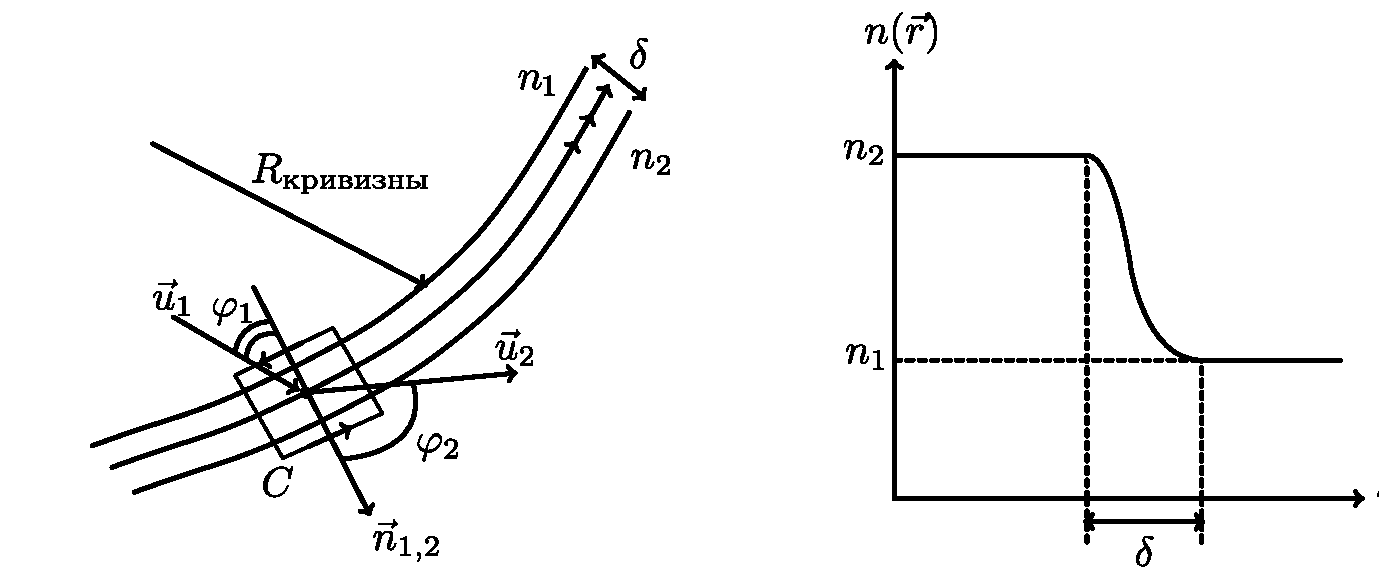
\includegraphics[width=0.8\textwidth]{/Users/vladbelousov/Desktop/Semestr_4-FP-NSU/ЭиО/Лекции_по_дням/image/66.pdf}
\end{center}

\[ \oint_{C} (\nabla \psi ,dl ) = 0  \Rightarrow n_2 (\vec{u }_ 2  ,\Delta \vec{l} ) + n_1 (\vec{u } _1 , - \Delta \vec{l} ) = 0 \] 

\[ n_2 \Delta l \sin  \varphi_2 = n_1 \Delta l \sin \varphi_1 \Rightarrow \boxed{n_1 \sin \varphi_1 = n_2 \sin  \varphi_2} \text{ - закон Снеллиуса}   \] 

\textbf{Гамильтонова форма уравнения луча: } 

\[ n (\vec{r } )\frac{d}{ds } \left(  n (\vec{r } ) \frac{d \vec{r } }{ds}  \right) = \nabla n \cdot n (\vec{r } ) \] 

\[ d \tau = \frac{ds}{d n(\vec{r } )} \Rightarrow \frac{d}{d \tau } \bigg( m , \kern-2cm \underbrace{\frac{d \vec{r } }{d \tau}}_{\text{скорость частице, двигающиеся вдоль луча } }  \kern-2cm \bigg)   =\nabla \frac{ n ^2  (\vec{r } )}{2 }  \] 

\[ \begin{cases}
    \displaystyle m \frac{d \vec{r } }{d \tau }  = \vec{ p } , \quad  \frac{ d \vec{ p } }{d \tau } =\vec{F } = - \nabla U = \nabla \frac{ n ^2 (\vec{r } )}{2 }  \\
    \displaystyle \frac{ d \vec{r } }{dt } = \frac{ \vec{p } }{m } \text{ ; Сохраняется полная энергия}   
\end{cases} \] 

\[ \frac{ p ^2 }{ 2 m } + U = \mathrm{const}    \]

\[ \frac{(\nabla \psi ) ^2 }{2 } -\frac{ n ^2 (\vec{r } )}{2 } =0 \text{ - уравнение эйконала}   \] 

\section{Вариационный принцип - принцип Ферма} 

\begin{center}
    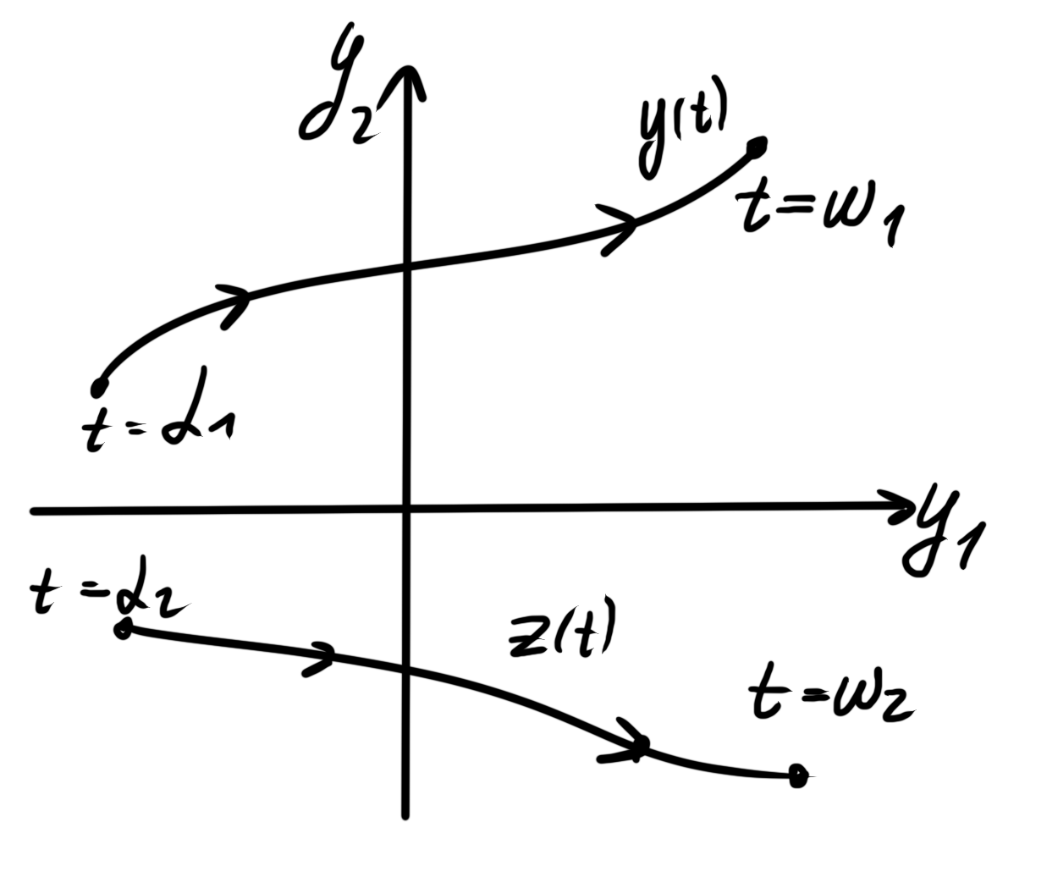
\includegraphics[width=0.3\textwidth]{/Users/vladbelousov/Desktop/Semestr_4-FP-NSU/ЭиО/Лекции_по_дням/image/67.png}
\end{center}

Оптический путь реального луча между точками \( p_1  \) и \( p_2  \) меньше или равен оптическому пути по \( \forall     \) другой траектории.

\[ \int_{ p_1 }^{p_2 } n (\vec{r } )d s = \int_{ p_1 }^{ p_2} \underbrace{ n (\vec{r } ) \sqrt{ \left( \frac{dx}{dt }     \right) ^2 + \left( \frac{dy}{dt }     \right) ^2  +\left( \frac{dz}{dt }     \right) ^2  }}_{\mathbb{L}(\vec{r }  ,\dot{ \vec{r}}  )} dt = \min  \] 

\[ \begin{aligned}
    \frac{d }{dt } \left(  \frac{\partial  L }{\dot{x } }  \right) &=   \frac{\partial  L }{x}  \to \frac{d}{dt } \left(  \frac{ 2 \dot{ x }  n (\vec{r } )}{ 2 \sqrt{\dot{ x } ^2 + \dot{ y } ^2 + \dot{ z } ^2 } }   \right) = \sqrt{\dot{ x } ^2 + \dot{ y } ^2 + \dot{ z } ^2}  \frac{\partial  n ( \vec{r } )}{\partial  x} \\ 
    \frac{d }{dt } \left(  \frac{\partial  L }{\dot{y } }  \right) &=  \frac{\partial  L }{y} \\
    \frac{d }{dt } \left(  \frac{\partial  L }{\dot{z } }  \right) &=   \frac{\partial  L }{z} 
\end{aligned} \] 

\[     \frac{d}{\sqrt{\dot{ x } ^2 + \dot{ y } ^2 + \dot{ z } ^2 }} \left(  \frac{\vec{e } _x \dot{ x }  n(\vec{r } )}{\sqrt{\dot{ x } ^2 + \dot{ y } ^2 + \dot{ z } ^2 }}  \right) = \vec{e } _x \frac{ \partial  n (\vec{r } )}{\partial  x } 
\] 

\[ \begin{array}{l|}
    \displaystyle \frac{d}{\sqrt{\dot{ x } ^2 + \dot{ y } ^2 + \dot{ z } ^2 }} \left(  \frac{\vec{e } _x \dot{ x }  n(\vec{r } )}{\sqrt{\dot{ x } ^2 + \dot{ y } ^2 + \dot{ z } ^2 }}  \right) =  \vec{e } _x \frac{ \partial  n (\vec{r } )}{\partial  x } \\
\end{array}   \] 

Примеры решений уравнений луча: 

1) Однородное пространство \( n(\vec{r } ) = \mathrm{const} = n_0  \) 

\[ \frac{d}{ds } \left( n_0 \frac{ d \vec{r } }{d s }     \right) = 0 \Rightarrow n_0 \frac{d \vec{r } }{ds} = \vec{a } \text{ - постоянные вектор}  \] 

\[ \vec{r } = \frac{ \vec{a } }{ n_0 }s + \vec{b }   \] 

\begin{center}
    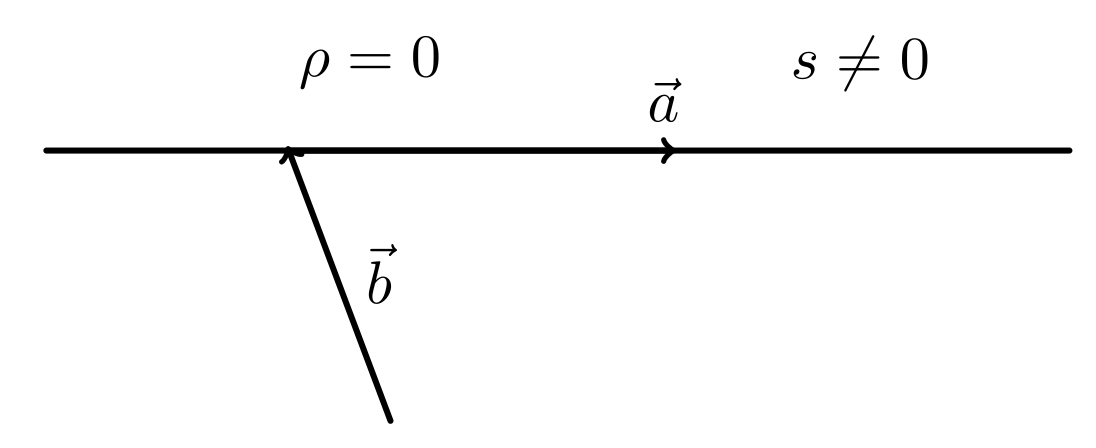
\includegraphics[width=0.5\textwidth]{/Users/vladbelousov/Desktop/Semestr_4-FP-NSU/ЭиО/Лекции_по_дням/image/90.png}
\end{center}

2) Движение луча в сферически симметричном распределении \( n(\vec{r } ) = n (r ) \) 

\[ \vec{p }  = n ( r ) \frac{ d \vec{r } }{ds}   \] 

Должен сохранятся момент импульса, проверим это:

\[ \frac{d}{ds } [\vec{r } \times  \vec{p } ] = \frac{d}{ds }  \left[ \vec{r } \times  n(r )\frac{d \vec{r } }{d s }  \right] = \underbrace{\left[  \frac{ d \vec{r } }{ ds }\times  n(r ) \frac{ d \vec{r } }{ds}   \right]}_{ = 0} + \underbrace{\bigg[ \vec{r } \times  \underbrace{\frac{d}{ds } \left( n(r ) \frac{ d \vec{r } }{ds}  \right)}_{= - \nabla n(r ) \sim \vec{e } _r} \bigg]}_{= 0}\] 

\begin{center}
    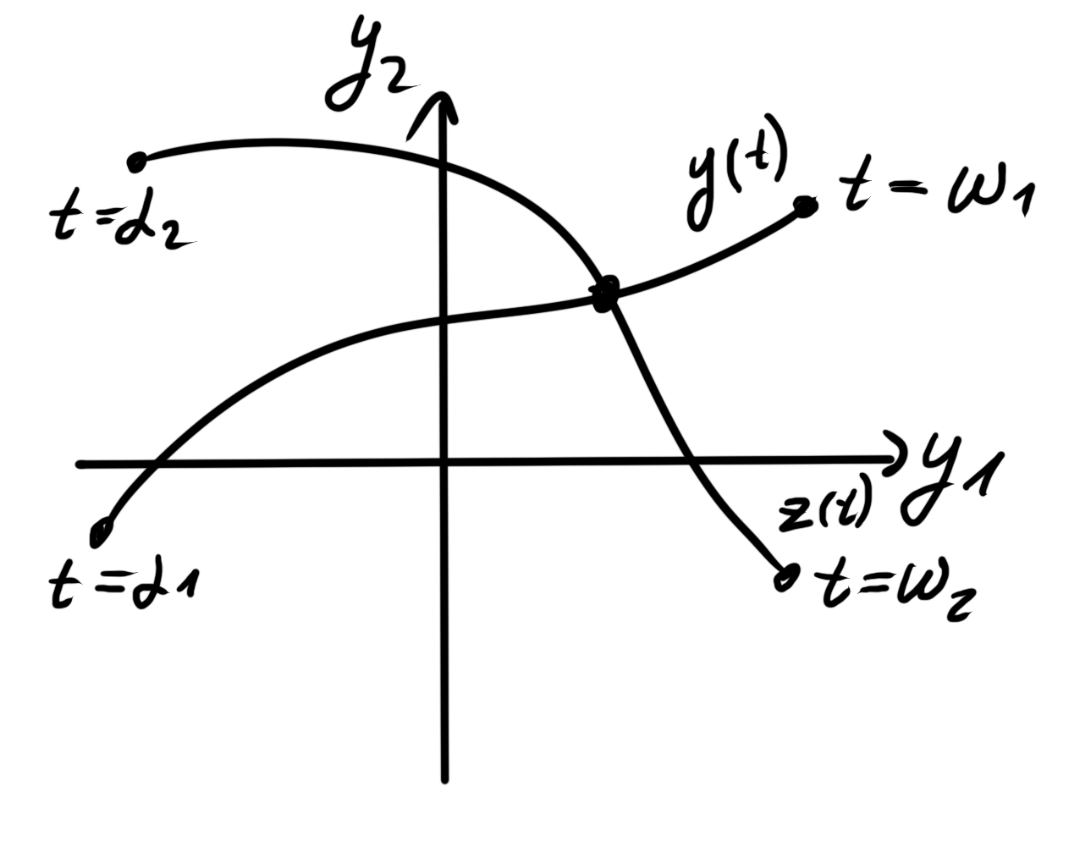
\includegraphics[width=0.7\textwidth]{/Users/vladbelousov/Desktop/Semestr_4-FP-NSU/ЭиО/Лекции_по_дням/image/68.png}
\end{center}

\[ \left\lvert [\vec{r } \times  n \frac{ d \vec{r } }{ds } ]  \right\rvert= \mathrm{const }  = \left\lvert [ \vec{r } _0 \times  \vec{u} ] \right\rvert = r_0 \sin \varphi_0 = \rho_0  \] 

Мираж

\begin{center}
    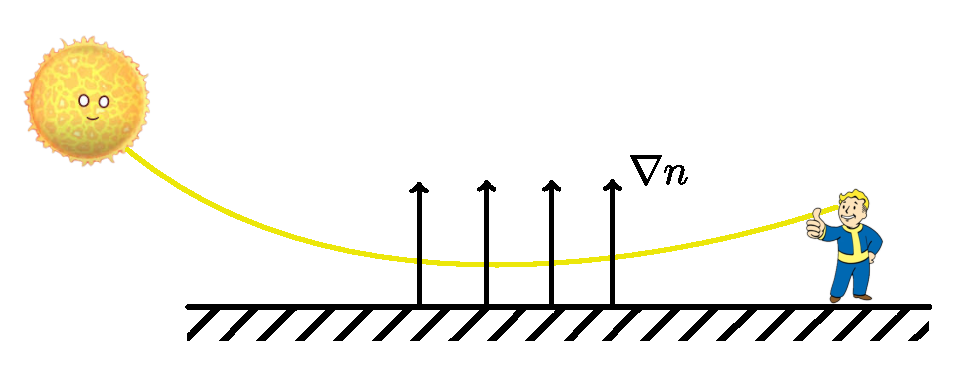
\includegraphics[width=0.8\textwidth]{/Users/vladbelousov/Desktop/Semestr_4-FP-NSU/ЭиО/Лекции_по_дням/image/69.pdf}
\end{center}

\[ T_{\text{в} } \sim 30^{\circ } C \quad T_{\text{п }  } \sim  100^{\circ } C    \] 

\[ T_{\text{песка} }\gg T_{\text{воздуха } }   \] 

\section{Оптические системы}

- состоят из тел с \( n = \mathrm{const}   \), в них лучи являются прямыми 

Преломление лучей на сферической поверхности

\begin{center}
    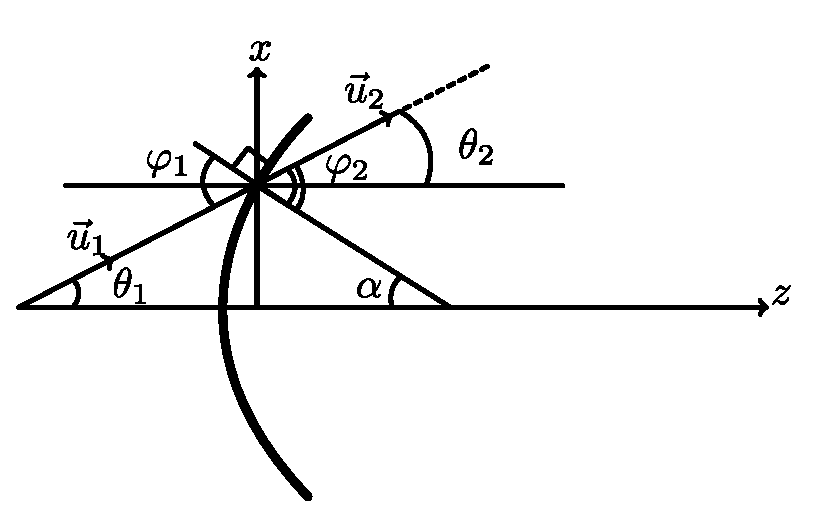
\includegraphics[width=0.6\textwidth]{/Users/vladbelousov/Desktop/Semestr_4-FP-NSU/ЭиО/Лекции_по_дням/image/70.pdf}
\end{center}



Используем приближение малых углов (параксиальное приближение)

\[ \theta_1 = \widehat{\vec{u } _1 \vec{e } _z }  \quad  \theta_2 = \widehat{\vec{u } _2 \vec{e } _z }     \] 

Правила:

1) Если луч удаляется от оси при движении слева направо, то \( \theta> 0  \), если приближается, то \( \theta<0 \) 

2) Если выпуклость сферической границы обращена  навстречу лучу (слева направо), то \( R>0 \), если наоборот, то \( R<0 \) 

Из закона Снеллиуса: 

\[ n_1 \sin \varphi_1 = n_2 \sin \varphi_2 \quad  (R \gg \lambda ) \] 

\[ n_1 \sin  (\theta_1 + \alpha ) = n_2 \sin (\theta_2 +\alpha ) \underset{\text{луча с линзой} }{\xrightarrow{x_1 \text{ - точка пересечения } }}    n_1\left( \theta_1 + \frac{x_1}{R}  \right) = n_2\left( \theta_2 + \frac{x_1}{R}  \right) \to   \]  

\[ \xrightarrow{\alpha = \mathrm{arcsin } \frac{x_1}{R } \approx \frac{x_1}{R}  } \theta_2 = \frac{n_1}{n_2 } \theta_1 - \left( 1 - \frac{n_1}{n_2}  \right) \frac{x_1}{R }  = \frac{n_1}{n_2 } \theta_1 - \frac{x_1}{F_{12}}      \] 

%%-------------------------------%%

% Закрытие документа, если файл компилируется отдельно
\ifdefined\mainfile
    % Если это основной файл, не нужно заканчивать документ
\else
    \end{document}
\fi